\documentclass{article}
\usepackage[utf8]{inputenc}
\usepackage[T1]{fontenc}
\usepackage{amsmath}
\usepackage{amsfonts}
\usepackage{amssymb}
\usepackage{graphicx}
\usepackage{float}
\usepackage{hyperref}
% Hide the link borders
\hypersetup{hidelinks}
\usepackage{geometry}
% Margins for A4 paper
\geometry{a4paper, margin=1.8cm}
\usepackage{enumitem}
% Spacing for itemize lists
\setlist[itemize]{itemsep=0.2em, topsep=0.2em, parsep=0pt, partopsep=0pt}
\setlength{\parindent}{0pt} % No paragraph indentation
\setlength{\emergencystretch}{2em} % Prevent overfull hboxes

\title{\textbf{Sprawozdanie z projektu z Mechatroniki} \\\textit{Termostat IOT z układem regulacji PID}}
\author{Mikołaj Kuryło s193743 \\Antonina Włodarczyk s197793}
\date{}

\begin{document}

\maketitle
\vspace{2cm}

\section{Cel projektu}

Celem projektu było stworzenie zdalnie sterowanego termostatu poprzez interfejs internetowy umożliwiający regulację temperatury w pomieszczeniu. System miał umożliwiać monitorowanie aktualnej temperatury, stanu grzania bądź chłodzenia oraz ustawienie żądanej temperatury. Dodatkowo, projekt zakładał implementację algorytmu regulacji PID w celu utrzymania stabilnej temperatury w pomieszczeniu. 

\begin{figure}[H]
    \centering
    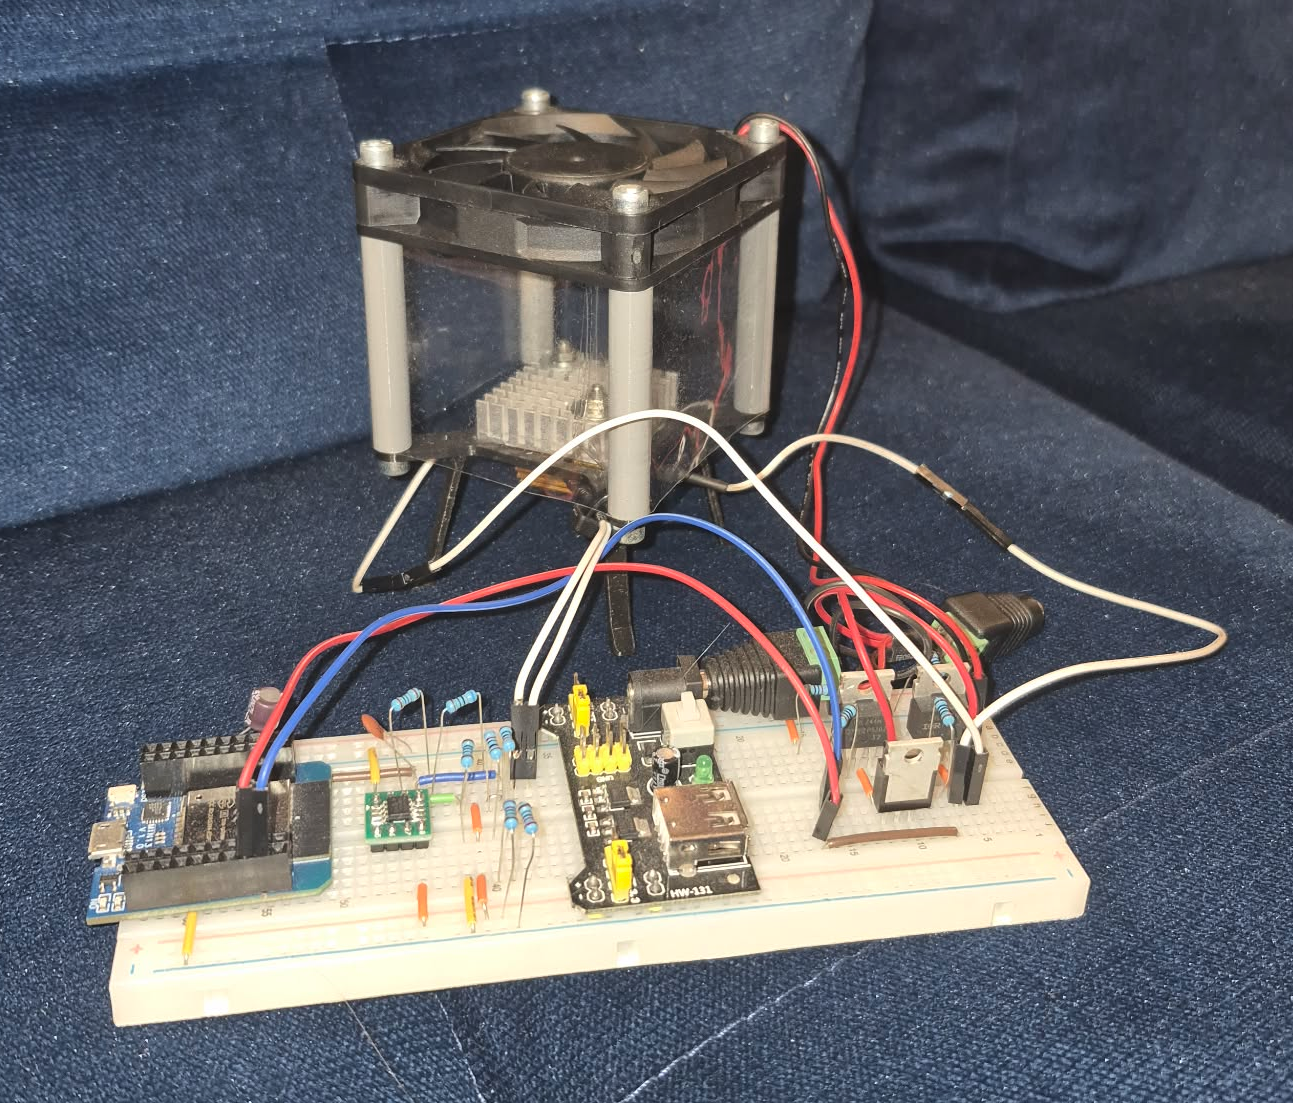
\includegraphics[width=0.5\textwidth]{img/termostat.png}
    \caption{Gotowy układ demonstracyjny}
\end{figure}

\section{Opis projektu}

Jako główną jednostkę wykonawczą całego systemu wykorzystano mikrokontroler ESP32 firmy Espressif, bogaty w liczne układy peryferyjne oraz biblioteki programistyczne. W ramach demonstracji działania systemu, zbudowano prostu układ kontrolny wykorzystujący rezystor grzewczy, wentylator chłodzący oraz termistor NTC pełniący rolę czujnika temperatury. Z racji działania termistora, przed jego podłączeniem do mikrokontrolera, zbadano jego charakterystykę w funkcji temperatury, poddano linearyzacji, a następnie zbudowano układ dzielnika napięcia ze wzmacniaczem operacyjnym w celu dopasowania sygnału do zakresu wejściowego mikrokontrolera (0-3.3V dla temperatur od 0 do 60 °C). Do bezprzewodowej komunikacji z systemem wykorzystano protokół Wi-Fi, a interfejs użytkownika został stworzony w formie strony internetowej dostępnej z poziomu przeglądarki.

\subsection{Układ elektroniczny i architektura systemu}

Sterowanie rezystorem grzewczym oraz wentylatorem chłodzącym odbywa się poprzez tranzystory MOSFET IRLZ44N, które umożliwiają wysterowanie urządzeń o większym poborze prądu oraz napięciu niż mikrokontroler jest w stanie zapewnić. W przypadku rezystora grzewczego sterowanie odbywa się poprzez modulację szerokości impulsu (PWM), natomiast w przypadku wentylatora chłodzącego zastosowano prosty włącz/wyłącz. 

\medskip
Termistor NTC jak wcześniej wspomniano, jest włączony w układ dzielnika napięcia, którego sygnał wyjściowy jest następnie podawany jako wejście nieodwracającego wzmacniacza operacyjnego MCP6002E, który pełni rolę bufora oraz wzmacniacza sygnału. Wzmacniacz operacyjny jest zasilany napięciem 3.3V, a jego wyjście jest podłączone do wejścia analogowego mikrokontrolera ESP32.

\begin{figure}[H]
    \centering
    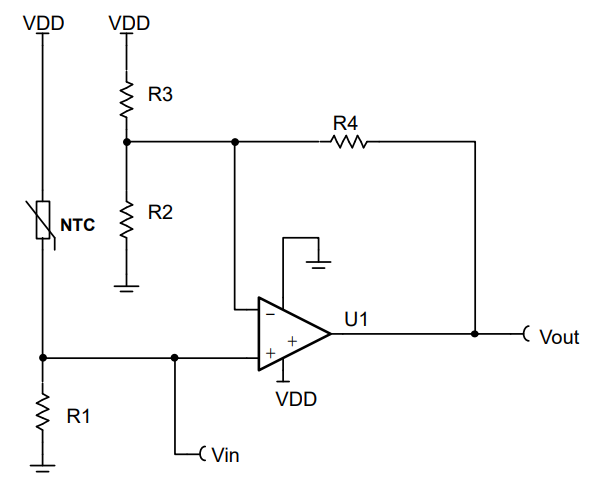
\includegraphics[width=0.4\textwidth]{img/uklad.png}
    \caption{Schemat układu elektronicznego sterowania termostatem}
\end{figure}

\subsection{Algorytm regulacji PID}

Oprogramowanie mikrokontrolera zostało zrealizowane w środowisku ESP-IDF w oparciu o system czasu rzeczywistego FreeRTOS, dzięki czemu odczyt temperatury, regulacja oraz obsługa serwera WWW działają jako niezależne, współbieżne zadania (\texttt{ntc\_readout\_task} oraz \texttt{regulator\_task}), komunikujące się poprzez współdzieloną strukturę \texttt{regulator\_t} chronioną mutexem, co zabezpiecza dostęp do danych przed sytuacjami wyścigu.

\medskip
Zadanie \texttt{ntc\_readout\_task} próbkuje przetwornik ADC z określoną częstotliwością, przelicza odczyt na temperaturę zgodnie z dwupunktową kalibracją liniową (napięcie $\rightarrow$ temperatura), a następnie zapisuje wynik do bufora cyklicznego. Zadanie regulacyjne odczytuje z tego bufora średnią ruchomą temperatury, co ogranicza wpływ szumu pomiarowego na działanie regulatora.

\medskip
Ponieważ obwód wykonawczy może wyłącznie grzać (rezystor grzewczy) lub wyłącznie chłodzić (wentylator), zastosowano regulację typu \emph{split-range} z pasmem martwym wokół zadanej wartości ($\pm \text{deadband}/2$):
\begin{itemize}
    \item gdy błąd regulacji $e = \text{setpoint} - T$ jest większy niż połowa pasma martwego -- aktywny jest wyłącznie regulator PID grzania, a wentylator chłodzący jest wyłączony,
    \item gdy błąd jest mniejszy niż $-\text{deadband}/2$ -- grzałka jest wyłączana, a wentylator załączany na stałe wypełnienie bez regulacji PID,
    \item wewnątrz pasma martwego oba wyjścia są wyłączone, a stan regulatora PID jest zerowany.
\end{itemize}
W każdej chwili aktywne jest tylko jedno z wyjść, a przy przełączaniu strony sterowania człon całkujący regulatora PID jest resetowany, co zapewnia łagodne wznowienie regulacji grzania przy kolejnym przekroczeniu progu.

\medskip
Regulator PID dla grzania został zaimplementowany w postaci równania:
\begin{equation}
    u(t) = K_p e(t) + K_i \int_0^t e(\tau)\, d\tau + K_d \frac{de(t)}{dt}
\end{equation}
z ograniczeniem wyjścia do zakresu $[0, 100]\%$ wypełnienia sygnału PWM oraz mechanizmem \emph{anti-windup} opartym o całkowanie warunkowe: jeżeli wyjście regulatora jest już nasycone na granicy zakresu, a kolejny krok błędu pogłębiałby to nasycenie, człon całkujący nie jest aktualizowany; całkowanie jest wznawiane natychmiast, gdy błąd zaczyna sprowadzać wyjście z powrotem w dopuszczalny zakres. Dzięki temu unika się klasycznego zjawiska narastania członu całkującego podczas nasycenia siłownika i wynikającego z niego przeregulowania po zmianie znaku błędu.

\medskip
Nastawy regulatora $K_p$, $K_i$, $K_d$ wyznaczono metodą Zieglera-Nicholsa w wariancie otwarto-pętlowym. Do wyznaczenia nastaw posłużono się dedykowanym zadaniem strojącym, które podaje na grzałkę skokowe wymuszenie o zadanym wypełnieniu, a następnie loguje przebieg temperatury w czasie aż do ustabilizowania się odczytu, osiągnięcia limitu czasu lub przekroczenia bezpiecznej temperatury. Z zarejestrowanego przebiegu odczytano wzmocnienie statyczne obiektu $K$, opóźnienie transportowe $L$ oraz stałą czasową $T$, na podstawie których wyznaczono nastawy według opisanych reguł:
\begin{equation}
    K_p = 1.2\,\frac{T}{K \cdot L}, \qquad T_i = 2L, \qquad K_i = \frac{K_p}{T_i}, \qquad T_d = 0.5L, \qquad K_d = K_p \cdot T_d
\end{equation}
Wyznaczone w ten sposób wartości zostały zapisane jako stałe w pliku nagłówkowym \texttt{regulator.h} i są wykorzystywane do obliczenia gotowych nastaw PID przy każdym uruchomieniu regulatora. Zadanie strojenia oraz zadanie regulacyjne nie mogą być uruchamiane jednocześnie, aktywne jest w danej chwili tylko jedno z nich.

\medskip
Niezależnie od działania regulatora PID zaimplementowano dodatkowe, nadrzędne zabezpieczenie programowe: jeśli uśredniona temperatura przekroczy wartość graniczną (50\textdegree C), grzałka jest natychmiast i bezwarunkowo wyłączana, wentylator załączany na pełne wypełnienie, a stan regulatora PID zerowany niezależnie od wyniku obliczeń. Pętla regulacyjna wykonywana jest cyklicznie ze stałym okresem.

\subsection{Interfejs użytkownika i komunikacja z systemem}

Komunikacja z użytkownikiem odbywa się za pośrednictwem wbudowanego serwera HTTP, uruchamianego na ESP32 po nawiązaniu połączenia Wi-Fi. Przy pierwszym uruchomieniu urządzenie sprawdza, czy zostało wcześniej sparowane z siecią. W przypadku braku konfiguracji, uruchamiany jest tryb provisioningu z własnym punktem dostępowym SoftAP, w przeciwnym razie urządzenie automatycznie łączy się ze skonfigurowaną siecią, z mechanizmem ponawiania próby połączenia w przypadku rozłączenia. Dodatkowo, w momencie uzyskania adresu IP, uruchamiana jest usługa mDNS, dzięki czemu panel jest dostępny pod stałym adresem \texttt{http://thermo.local} bez konieczności znajomości adresu IP urządzenia w sieci lokalnej.

\medskip
Dostęp do parametrów regulatora z poziomu serwera odbywa się poprzez strukturę pośredniczącą \texttt{server\_regulator\_t}, zawierającą wskaźniki do bieżącej temperatury i wyjść regulatora oraz wskaźniki na funkcje \texttt{get}/\texttt{set}, które wewnętrznie korzystają z tego samego mutexa co zadanie regulacyjne (\texttt{regulator\_get\_params}/\texttt{regulator\_set\_params}), zapewniając bezpieczny odczyt i zapis danych współdzielonych między zadaniem obsługi HTTP a zadaniem regulacji.

\medskip
Panel użytkownika (rys. \ref{fig:panel}) to responsywna strona internetowa, wyświetlająca aktualną oraz zadaną temperaturę, tryb pracy (grzanie/chłodzenie/bezczynność) wraz z procentowym wypełnieniem obu wyjść, formularz pozwalający ustawić nową temperaturę zadaną i pasmo martwe. Strona cyklicznie odpytuje serwer, aktualizując wyświetlane wartości oraz wskaźnik stanu połączenia; w przypadku braku odpowiedzi serwera pola formularza są blokowane, a wskaźnik połączenia sygnalizuje błąd. Zapis nowych nastaw następuje po zatwierdzeniu formularza, poprzez wysłanie żądania \texttt{POST} z danymi w formacie JSON, po czym stan panelu jest natychmiast odświeżany.

\begin{figure}[H]
    \centering
    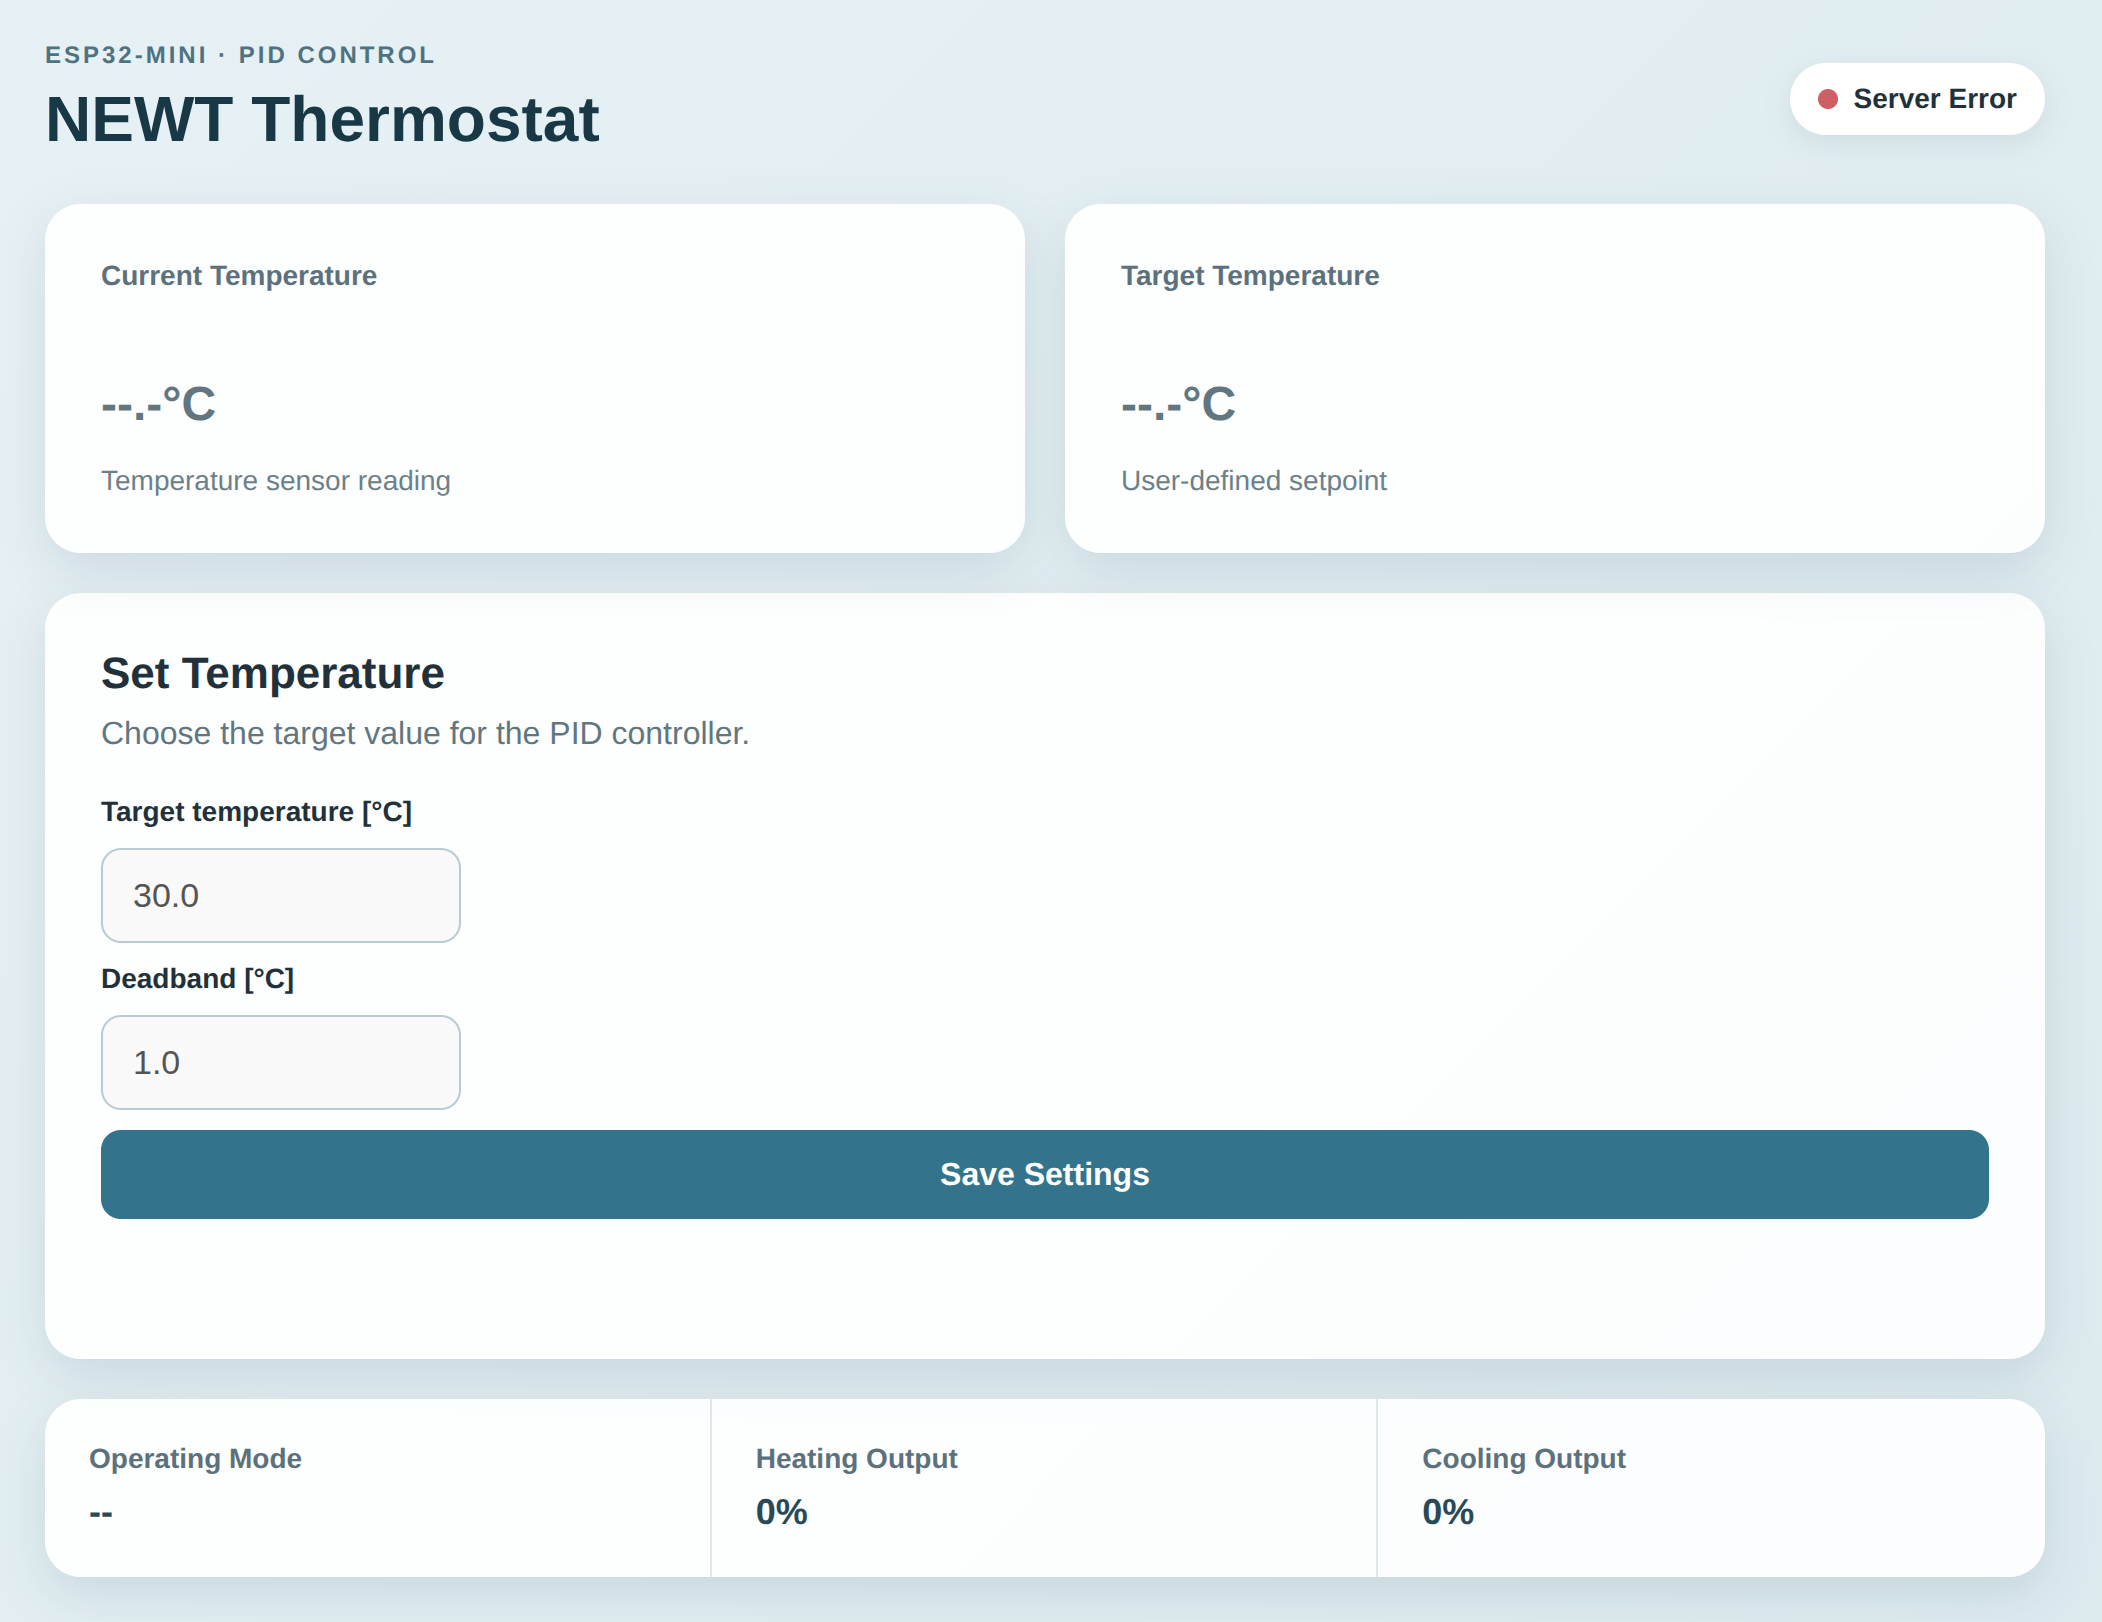
\includegraphics[width=0.8\textwidth]{img/panel.png}
    \caption{Panel sterowania termostatem dostępny przez przeglądarkę}
    \label{fig:panel}
\end{figure}

\end{document}